\documentclass{article}
\usepackage{polski}
\usepackage{float}
\usepackage{adjustbox}
\usepackage{xcolor}
\usepackage{amssymb}
\usepackage[shortlabels]{enumitem}
\usepackage{graphicx}
\usepackage{amsmath}
\graphicspath{ {./img/} }

\title{Sprawozdanie 2 - Obliczenia Naukowe}
\author{Michał Kallas}
\date{9 listopada 2024}

\begin{document}

\maketitle

\section{Zadanie 1}
\subsection{Opis problemu}
Powtórzyć zadanie 5. z listy 1, ale usunąć ostatnią 9 z $x_4$ i ostatnią 7 z $x_5$. Sprawdzić jaki wpływ na wyniki mają
niewielkie zmiany danych.\\

\noindent Oryginalne wektory:

\begin{description}
    \item $x = [2.718281828, -3.141592654, 1.414213562, 0.577215664\textcolor{red}{9}, 0.301029995\textcolor{red}{7}]$
    \item $y = [1486.2497, 878366.9879, -22.37492, 4773714.647, 0.000185049]$
\end{description}

\noindent Wektor $x$ po zmianach:

\begin{description}
    \item $x' = [2.718281828, -3.141592654, 1.414213562, 0.577215664, 0.301029995]$
\end{description}

\subsection{Wyniki}
Poprawny wynik to $-1.00657107000000 * 10^{-11}$. Poniżej otrzymane wyniki eksperymentalne:

\begin{table}[H]
\begin{adjustbox}{center}
\begin{tabular}{|c|c|c|c|c|c|}
    \hline
    Typ & Wektory & Metoda a & Metoda b & Metoda c & Metoda d\\
    \hline
    Float32 & $x$, $y$ & -0.4999443 & -0.4543457 & -0.5 & -0.5\\
    \hline
    Float32 & $x'$, $y$ & -0.4999443 & -0.4543457 & -0.5 & -0.5\\
    \hline
    Float64 & $x$, $y$ & 1.0251881368296672e-10 & -1.5643308870494366e-10 & 0.0 & 0.0\\
    \hline
    Float64 & $x'$, $y$ & -0.004296342739891585 & -0.004296342998713953 & -0.004296342842280865 & -0.004296342842280865\\
    \hline
\end{tabular}
\end{adjustbox}
\caption{Porównanie wyników 4 algorytmów do obliczenia iloczynu skalarnego dla wektorów $x$ i $y$ oraz $x'$ i $y$.}
\end{table}

\subsection{Obserwacje i wnioski}
Wyniki dla typu \texttt{Float32} są dokładnie takie same dla nowego wektoru $x$. Wiąże się to ze zbyt małą precyzją tej
arytmetyki.

Z kolei dla bardziej precyzyjnego typu \texttt{Float64} możemy zobaczyć dużą rozbieżność wyników pomiędzy starym, a
nowym wektorem $x$, mimo małej różnicy danych. To oznacza, że zadanie jest źle uwarunkowane.

\section{Zadanie 2}
\subsection{Opis problemu}
Narysować wykres funkcji $f(x) = e^{x}\ln(1 + e^{-x})$ w co najmniej dwóch dowolnych
programach do wizualizacji. Następnie policzyć granicę funkcji $\lim_{x \to \infty} f(x)$. Porównać
wykres funkcji z policzoną granicą. Wyjaśnić zjawisko.

\subsection{Wyniki}
\begin{figure}[H]
\centering
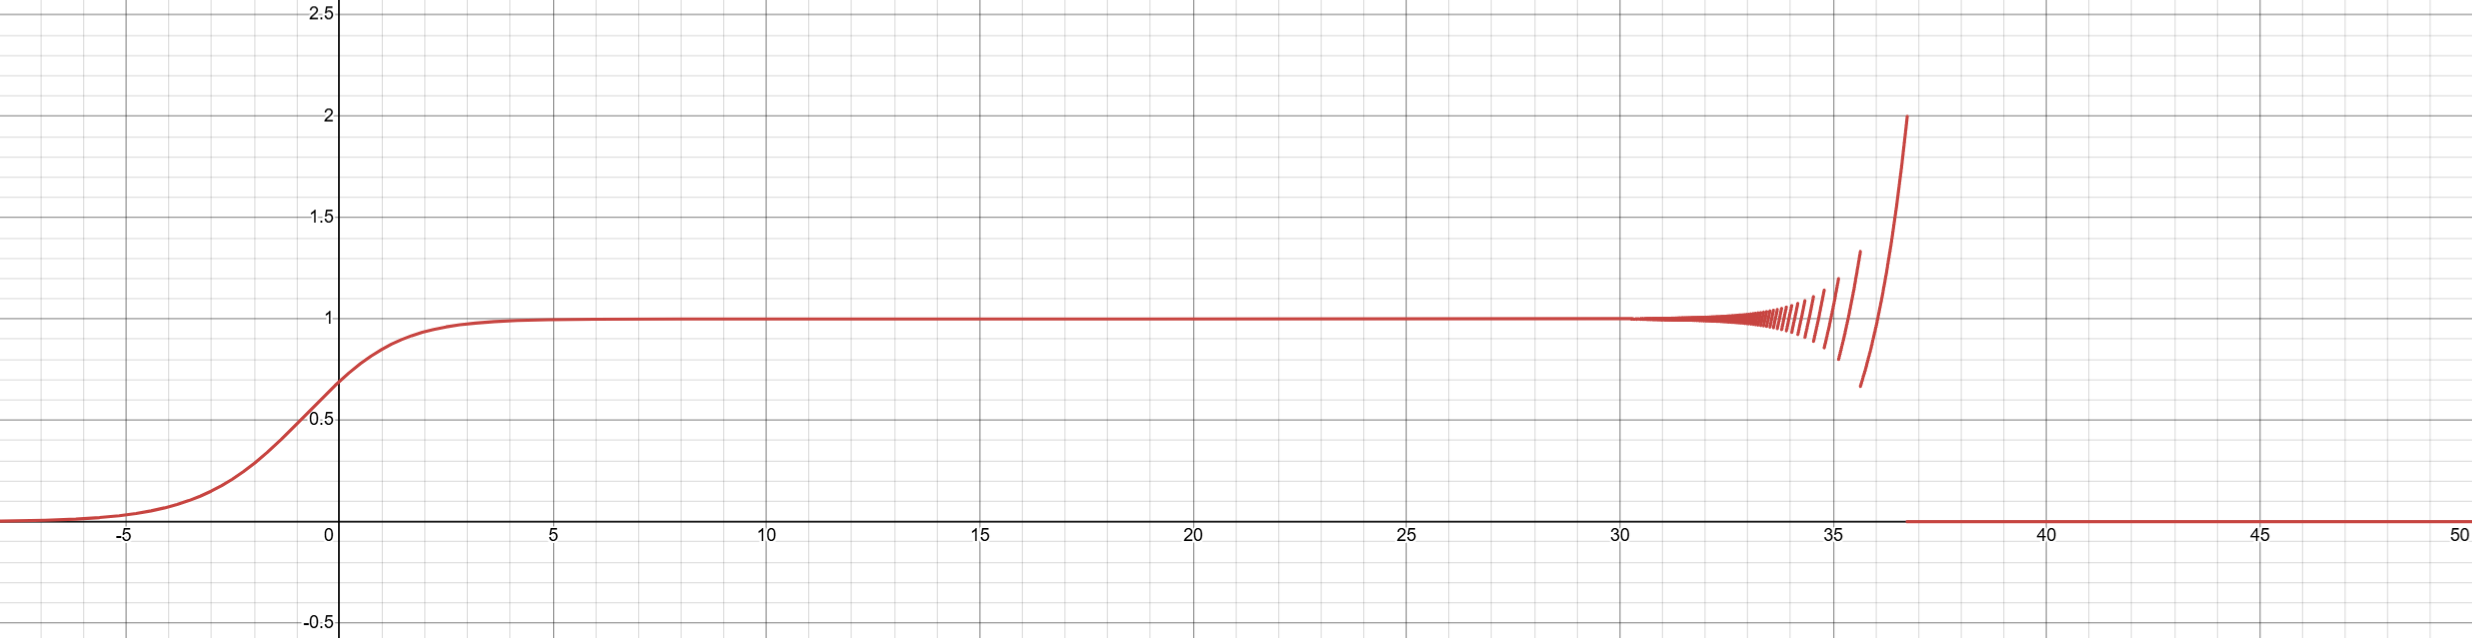
\includegraphics[width=\textwidth]{Desmos.png}
\caption{Wykres $f(x) = e^{x}\ln(1 + e^{-x})$ w Desmos.}
\end{figure}

\begin{figure}[H]
\centering
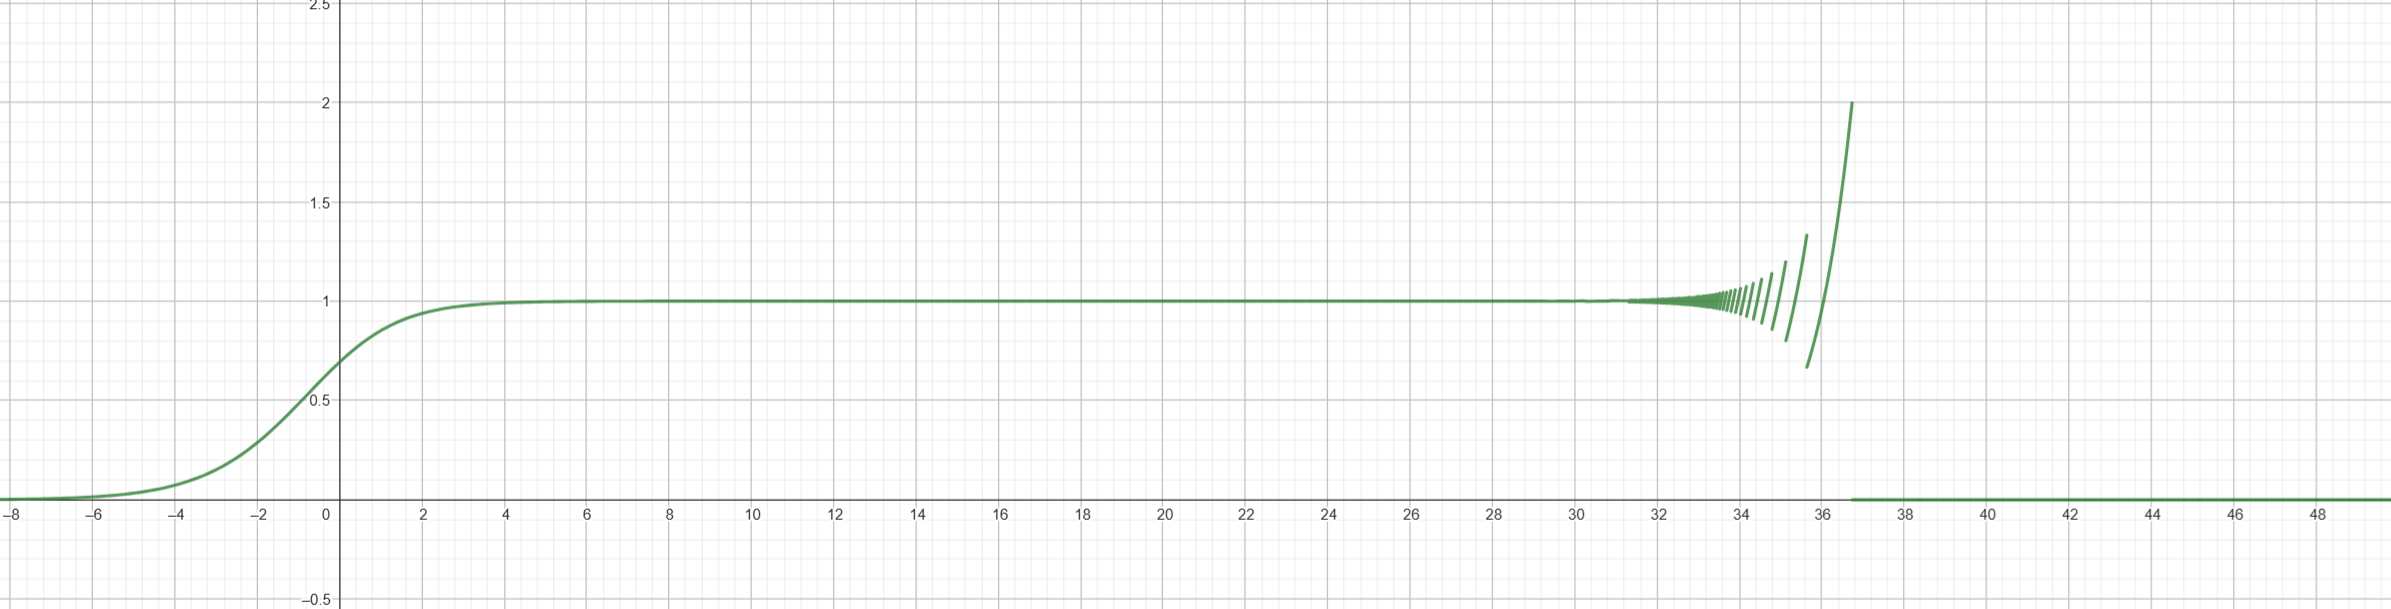
\includegraphics[width=\textwidth]{GeoGebra.png}
\caption{Wykres $f(x) = e^{x}\ln(1 + e^{-x})$ w GeoGebra.}
\end{figure}

Wyliczona granica:
$$\lim_{x \to \infty} f(x) = \lim_{x \to \infty} e^{x}\ln(1 + e^{-x}) = 1$$

\subsection{Obserwacje i wnioski}
Wykresy od pewnego momentu nie zgadzają się z faktycznymi wartościami $f(x)$. Zaczynają się nietypowo zachowywać dla
$x > 30$, gdzie występują duże wahania wyników. Powodem takiego stanu rzeczy jest mnożenie $e^{x}$ przez $\ln(1 + e^{-x})$,
gdzie dla odpowiednio dużych $x$ pierwszy czynnik staje się bardzo duży, a drugi bardzo mały. Tego typu operacje
prowadzą do poważnych błędów.

Dla $x$ w okoliach 36 wartość funkcji spada do zera. Wynika to z tego, że $\ln(1 + e^{-x}) \approx 0$, co zeruje całe
wyrażenie. To nie pokrywa się z wyliczoną granicą funkcji, bo jej wartości powinny dążyć do 1.

Bardzo małe różnice w danych spowodowały duże różnice w wyniku, a więc zadanie jest źle uwarunkowane.

\section{Zadanie 3}
\subsection{Opis problemu}
Rozwiązać układ równań liniowych $Ax = b$ dla danej macierzy współczynników $A \in \mathbb{R}^{n \times n}$ i wektora prawych stron
$b \in \mathbb{R}^{n}$ Porównać zastosowane metody pod względem błędów względnych. Macierz A ma być tworzona na dwa sposoby:
\begin{enumerate}[(a)]
    \item $A = H_n$, gdzie $H_n$ jest macierzą Hilberta stopnia $n$
    \item $A = R_n$, gdzie $R_n$ jest losową macierzą stopnia $n$ z zadanym wskaźnikiem uwarunkowania $c$
\end{enumerate}
Wektor $b$ zadany jest następująco: $b = Ax$, gdzie $x = (1, ..., 1)^{T}$. Dzięki temu znamy dokładne rozwiązanie dla
$A$ i $b$.
Układ równań należy rozwiązać danymi metodami:
\begin{enumerate}[(a)]
    \item metodą eliminacji Gausa, czyli $x = A \setminus b$
    \item metodą macierzy odwrotnej, czyli $x = A^{-1}b$
\end{enumerate}
Eksperymenty wykonać dla macierzy Hilberta $H_n$ z rosnącym stopniem $n > 1$ oraz dla macierzy losowej
$R_n, n = 5, 10, 20$ z rosnącym wskaźnikiem uwarunkowania $c = 1, 10, 10^{3}, 10^{7}, 10^{12}, 10^{16}$.

\subsection{Wyniki}
\begin{table}[H]
\begin{adjustbox}{center}
\begin{tabular}{|c|c|c|c|c|}
    \hline
    $n$ & $cond(A)$ & $rank(A)$ & Błąd metody Gaussa & Błąd metody inwersji\\
    \hline
    1 & 1.0 & 1 & 0.0 & 0.0\\
    \hline
    2 & 19.28147006790397 & 2 & 5.661048867003676e-16 & 1.4043333874306803e-15\\
    \hline
    3 & 524.0567775860644 & 3 & 8.022593772267726e-15 & 0.0\\
    \hline
    4 & 15513.73873892924 & 4 & 4.137409622430382e-14 & 0.0\\
    \hline
    5 & 476607.2502425855 & 5 & 1.6828426299227195e-12 & 3.3544360584359632e-12\\
    \hline
    6 & 1.4951058642254734e7 & 6 & 2.618913302311624e-10 & 2.0163759404347654e-10\\
    \hline
    7 & 4.753673567446793e8 & 7 & 1.2606867224171548e-8 & 4.713280397232037e-9\\
    \hline
    8 & 1.5257575538060041e10 & 8 & 6.124089555723088e-8 & 3.07748390309622e-7\\
    \hline
    9 & 4.9315375594102344e11 & 9 & 3.8751634185032475e-6 & 4.541268303176643e-6\\
    \hline
    10 & 1.602441698742836e13 & 10 & 8.67039023709691e-5 & 0.0002501493411824886\\
    \hline
    11 & 5.222701316549833e14 & 10 & 0.00015827808158590435 & 0.007618304284315809\\
    \hline
    12 & 1.7515952300879806e16 & 11 & 0.13396208372085344 & 0.258994120804705\\
    \hline
    13 & 3.1883950689209334e18 & 11 & 0.11039701117868264 & 5.331275639426837\\
    \hline
    14 & 6.200786281355982e17 & 11 & 1.4554087127659643 & 8.71499275104814\\
    \hline
    15 & 3.67568286586649e17 & 12 & 4.696668350857427 & 7.344641453111494\\
    \hline
\end{tabular}
\end{adjustbox}
\caption{Wartości wskaźnika uwarunkowania i rzędu macierzy {$H_n$} oraz błędy względne rozwiązań układu równań metodami Gaussa i z macierzą odwrotną.}
\end{table}

\begin{table}[H]
\begin{adjustbox}{center}
\begin{tabular}{|c|c|c|c|c|}
    \hline
    $n$ & $c$ & $rank(A)$ & Błąd metody Gaussa & Błąd metody inwersji\\
    \hline
    5 & 1.0 & 5 & 3.0606736594252445e-16 & 2.275280134513746e-16\\
    \hline
    5 & 10.0 & 5 & 1.2161883888976237e-16 & 1.4895204919483638e-16\\
    \hline
    5 & 1000.0 & 5 & 6.8830246068992106e-15 & 1.1655121101003682e-14\\
    \hline
    5 & 1.0e7 & 5 & 1.8433912490050538e-10 & 1.4317191526598063e-10\\
    \hline
    5 & 1.0e12 & 5 & 4.0271506137124706e-5 & 4.0414925152527825e-5\\
    \hline
    5 & 1.0e16 & 4 & 1.1102230246251565e-16 & 0.02115773708005347\\
    \hline
    10 & 1.0 & 10 & 2.4575834280036907e-16 & 3.0606736594252445e-16\\
    \hline
    10 & 10.0 & 10 & 3.4932351950072765e-16 & 3.665417751368233e-16\\
    \hline
    10 & 1000.0 & 10 & 1.8392579358722525e-14 & 2.6731071956605676e-14\\
    \hline
    10 & 1.0e7 & 10 & 1.672423868802004e-10 & 1.332910952506047e-10\\
    \hline
    10 & 1.0e12 & 10 & 1.4391864685145854e-5 & 1.0065760097123466e-5\\
    \hline
    10 & 1.0e16 & 9 & 0.01264020487412138 & 0.03992264919036816\\
    \hline
    20 & 1.0 & 20 & 6.483170143248366e-16 & 5.159850341939109e-16\\
    \hline
    20 & 10.0 & 20 & 5.347542221830666e-16 & 2.9893669801409083e-16\\
    \hline
    20 & 1000.0 & 20 & 3.1243567653618664e-14 & 2.9734251634904414e-14\\
    \hline
    20 & 1.0e7 & 20 & 3.967040176688922e-10 & 3.761993759834402e-10\\
    \hline
    20 & 1.0e12 & 20 & 1.650912083708681e-5 & 1.6620959308749998e-5\\
    \hline
    20 & 1.0e16 & 19 & 0.06915639868517645 & 0.06664947595151573\\
    \hline
\end{tabular}
\end{adjustbox}
\caption{Wartości wskaźnika uwarunkowania $c$ i rzędu macierzy {$R_n$} oraz błędy względne rozwiązań układu równań metodami Gaussa i z macierzą odwrotną.}
\end{table}

\subsection{Obserwacje i wnioski}
Dla macierzy Hilberta wskaźniki uwarunkowania i błędy względne dla obu metod szybko osiągają wysokie wartości. Widać,
że im większy wskaźnik uwarunkowania, tym większy błąd. W tym przypadku metoda Gaussa okazała się bardziej skuteczna -
w większości przypadków pozwoliła osiągnąć dokładniejsze wyniki.

W przypadku macierzy losowych o ustalonym wskaźniku uwarunkowania, błędy dla obu metod są mniejsze. Są na tyle zbliżone,
że ciężko jest wyłonić faworyta. Ponownie możemy zauważyć, że im większy wskaźnik uwarunkowania, tym większy błąd.
Widać, że błędy są podobnego rzędu dla macierzy o tych samych wskaźnikach uwarunkowania, ale różnych rozmiarach.

Możemy wywnioskować, że zadanie obliczenia układu równań $Ax = b$ dla macierzy Hilberta jest źle uwarunkowane.
Zadanie pokazuje nam to jak istotny jest wskaźnik uwarunkowania i że bezpośrednio przekłada się on na błędy.

\section{Zadanie 4}
\subsection{Opis problemu}
Dany jest ,,złośliwy wielomian'' Wilkinsona:
$$p(x) = \prod_{i = 1}^{20}$$
$P$ jest postacią naturalną wielomianu Wilkinsona $p$. Należy:

\begin{enumerate}[(a)]
    \item Obliczyć pierwiastki wielomianu $P$. Następnie sprawdzić obliczone pierwiastki \( z_k \),
    \( 1 \leq k \leq 20 \), obliczając \( |P(z_k)| \), \( |p(z_k)| \) i \( |z_k - k| \). Wyjaśnić rozbieżności.

    \item Powtórzyć eksperyment Wilsona marginalnie zaburzając jeden ze współczynników wielomianu. Odejmiemy od
    $a_{19} = -210$ wartość $2^{-23}$.
\end{enumerate}

\subsection{Wyniki}
\begin{table}[H]
\begin{adjustbox}{center}
\begin{tabular}{|c|c|c|c|c|}
    \hline
    $k$ & $z_k$ & $|P(z_k)|$ & $|p(z_k)|$ & $ |z_k - k|$\\
    \hline
    1 & 0.9999999999996989 & 35696.50964788257 & 5.518479490350445e6 & 3.0109248427834245e-13\\
    \hline
    2 & 2.0000000000283182 & 176252.60026668405 & 7.37869762990174e19 & 2.8318236644508943e-11\\
    \hline
    3 & 2.9999999995920965 & 279157.6968824087 & 3.3204139316875795e20 & 4.0790348876384996e-10\\
    \hline
    4 & 3.9999999837375317 & 3.0271092988991085e6 & 8.854437035384718e20 & 1.626246826091915e-8\\
    \hline
    5 & 5.000000665769791 & 2.2917473756567076e7 & 1.8446752056545688e21 & 6.657697912970661e-7\\
    \hline
    6 & 5.999989245824773 & 1.2902417284205095e8 & 3.320394888870117e21 & 1.0754175226779239e-5\\
    \hline
    7 & 7.000102002793008 & 4.805112754602064e8 & 5.423593016891273e21 & 0.00010200279300764947\\
    \hline
    8 & 7.999355829607762 & 1.6379520218961136e9 & 8.262050140110275e21 & 0.0006441703922384079\\
    \hline
    9 & 9.002915294362053 & 4.877071372550003e9 & 1.196559421646277e22 & 0.002915294362052734\\
    \hline
    10 & 9.990413042481725 & 1.3638638195458128e10 & 1.655260133520688e22 & 0.009586957518274986\\
    \hline
    11 & 11.025022932909318 & 3.585631295130865e10 & 2.24783329792479e22 & 0.025022932909317674\\
    \hline
    12 & 11.953283253846857 & 7.533332360358197e10 & 2.886944688412679e22 & 0.04671674615314281\\
    \hline
    13 & 13.07431403244734 & 1.9605988124330817e11 & 3.807325552826988e22 & 0.07431403244734014\\
    \hline
    14 & 13.914755591802127 & 3.5751347823104315e11 & 4.612719853150334e22 & 0.08524440819787316\\
    \hline
    15 & 15.075493799699476 & 8.21627123645597e11 & 5.901011420218566e22 & 0.07549379969947623\\
    \hline
    16 & 15.946286716607972 & 1.5514978880494067e12 & 7.010874106897764e22 & 0.05371328339202819\\
    \hline
    17 & 17.025427146237412 & 3.694735918486229e12 & 8.568905825736165e22 & 0.025427146237412046\\
    \hline
    18 & 17.99092135271648 & 7.650109016515867e12 & 1.0144799361044434e23 & 0.009078647283519814\\
    \hline
    19 & 19.00190981829944 & 1.1435273749721195e13 & 1.1990376202371257e23 & 0.0019098182994383706\\
    \hline
    20 & 19.999809291236637 & 2.7924106393680727e13 & 1.4019117414318134e23 & 0.00019070876336257925\\
    \hline
\end{tabular}
\end{adjustbox}
\caption{Wyniki eksperymentu dla oryginalnego wielomianu.}
\end{table}

\begin{table}[H]
\begin{adjustbox}{center}
\begin{tabular}{|c|c|c|c|c|}
    \hline
    $k$ & $z_k$ & $|P(z_k)|$ & $|p(z_k)|$ & $ |z_k - k|$\\
    \hline
    1 & 0.9999999999998357 + 0.0im & 20259.872313418207 & 19987.872313406842 & 1.6431300764452317e-13\\
    \hline
    1 & 0.9999999999998357 + 0.0im & 20259.872313418207 & 3.0131001276845885e6 & 1.6431300764452317e-13\\
    \hline
    2 & 2.0000000000550373 + 0.0im & 346541.4137593836 & 7.37869763029606e19 & 5.503730804434781e-11\\
    \hline
    3 & 2.99999999660342 + 0.0im & 2.2580597001197007e6 & 3.320413920110016e20 & 3.3965799062229962e-9\\
    \hline
    4 & 4.000000089724362 + 0.0im & 1.0542631790395478e7 & 8.854437817429642e20 & 8.972436216225788e-8\\
    \hline
    5 & 4.99999857388791 + 0.0im & 3.757830916585153e7 & 1.844672697408419e21 & 1.4261120897529622e-6\\
    \hline
    6 & 6.000020476673031 + 0.0im & 1.3140943325569446e8 & 3.320450195282313e21 & 2.0476673030955794e-5\\
    \hline
    7 & 6.99960207042242 + 0.0im & 3.939355874647618e8 & 5.422366528916004e21 & 0.00039792957757978087\\
    \hline
    8 & 8.007772029099446 + 0.0im & 1.184986961371896e9 & 8.289399860984408e21 & 0.007772029099445632\\
    \hline
    9 & 8.915816367932559 + 0.0im & 2.2255221233077707e9 & 1.160747250177049e22 & 0.0841836320674414\\
    \hline
    10 & 10.095455630535774 - 0.6449328236240688im & 1.0677921232930157e10 & 1.7212892853670706e22 & 0.6519586830380407\\
    \hline
    11 & 10.095455630535774 + 0.6449328236240688im & 1.0677921232930157e10 & 1.7212892853670706e22 & 1.1109180272716561\\
    \hline
    12 & 11.793890586174369 - 1.6524771364075785im & 3.1401962344429485e10 & 2.8568401004080956e22 & 1.665281290598479\\
    \hline
    13 & 11.793890586174369 + 1.6524771364075785im & 3.1401962344429485e10 & 2.8568401004080956e22 & 2.0458202766784277\\
    \hline
    14 & 13.992406684487216 - 2.5188244257108443im & 2.157665405951858e11 & 4.934647147686795e22 & 2.518835871190904\\
    \hline
    15 & 13.992406684487216 + 2.5188244257108443im & 2.157665405951858e11 & 4.934647147686795e22 & 2.7128805312847097\\
    \hline
    16 & 16.73074487979267 - 2.812624896721978im & 4.850110893921027e11 & 8.484694713563005e22 & 2.9060018735375106\\
    \hline
    17 & 16.73074487979267 + 2.812624896721978im & 4.850110893921027e11 & 8.484694713563005e22 & 2.825483521349608\\
    \hline
    18 & 19.5024423688181 - 1.940331978642903im & 4.557199223869993e12 & 1.3181947820607215e23 & 2.4540214463129764\\
    \hline
    19 & 19.5024423688181 + 1.940331978642903im & 4.557199223869993e12 & 1.3181947820607215e23 & 2.0043294443099486\\
    \hline
    20 & 20.84691021519479 + 0.0im & 8.756386551865696e12 & 1.5911084081430876e23 & 0.8469102151947894\\
    \hline
\end{tabular}
\end{adjustbox}
\caption{Wyniki eksperymentu dla marginalnie zaburzonego wielomianu.}
\end{table}

\begin{table}[H]
\begin{adjustbox}{center}
\begin{tabular}{|c|c|c|}
    \hline
    $k$ & $|P(k)|$ & $|p(k)|$\\
    \hline
    1 & 0.0 & 0\\
    \hline
    2 & 8192.0 & 0\\
    \hline
    3 & 27648.0 & 0\\
    \hline
    4 & 622592.0 & 0\\
    \hline
    5 & 2.176e6 & 0\\
    \hline
    6 & 8.84736e6 & 0\\
    \hline
    7 & 2.4410624e7 & 0\\
    \hline
    8 & 5.89824e7 & 0\\
    \hline
    9 & 1.45753344e8 & 0\\
    \hline
    10 & 2.27328e8 & 0\\
    \hline
    11 & 4.79074816e8 & 0\\
    \hline
    12 & 8.75003904e8 & 0\\
    \hline
    13 & 1.483133184e9 & 0\\
    \hline
    14 & 2.457219072e9 & 0\\
    \hline
    15 & 3.905712e9 & 0\\
    \hline
    16 & 6.029312e9 & 0\\
    \hline
    17 & 9.116641408e9 & 0\\
    \hline
    18 & 1.333988352e10 & 0\\
    \hline
    19 & 1.9213101568e10 & 0\\
    \hline
    20 & 2.7193344e10 & 0\\
    \hline
\end{tabular}
\end{adjustbox}
\caption{Wyniki wielomianów $P$(niezaburzony) i $p$ dla dokładnych pierwiastków.}
\end{table}

\subsection{Obserwacje i wnioski}
Wyliczone wartości pierwiastków dla niezaburzonego wielomianu nie pokrywają się z tymi dokładnymi, jednak są bardzo
zbliżone. Każdy błąd bezwględny $|z_k - k| < 0.1$. Mimo tego, wartości wielomianów dla niedokładnie wyliczonych
pierwiastków są ogromne. Wskazuje to na to, że zadanie wyznaczenia pierwiastków dla wielomianu Wilkinsona jest źle
uwarunkowane.

Arytmetyka \texttt{Float64} nie pozwala nam dokładnie przechować $P$ ze względu na ograniczoną precyzję. Niemożliwe do
dokładnego przechowania są te największe współczynniki. Z tego względu, nawet dla dokładnych pierwiastków $P(k)$ nie
zwraca 0, w przeciwieństwie do $p(k)$.

Marginalna zmiana w $P$ doprowadziła do większego błędu i pojawienia się rozwiązań zespolonych. To po raz kolejny
pokazuje, że zadanie wyznaczenia pierwiastków dla wielomianu Wilkinsona jest źle uwarunkowane.

\section{Zadanie 5}
\subsection{Opis problemu}
Rozważmy równanie rekurencyjne, reprezentujące model wzrostu populacji:
$$p_{n+1} := p_n + rp_n(1 - p_n)$$

\noindent Należy wyznaczyć 40 wyrazów tego równania dla $p_0 = 0.01$ i $r = 3$ na 3 sposoby:
\begin{enumerate}
    \item Dla typu \texttt{Float32}
    \item Dla typu \texttt{Float32}, obcinając wartość $p_{10}$ do 3 miejsc po przecinku i następnie kontynuując iteracje
    \item Dla typu \texttt{Float64}
\end{enumerate}

\subsection{Wyniki}
\begin{table}[H]
\begin{adjustbox}{center}
\begin{tabular}{|c|c|c|c|}
    \hline
    $n$ & Float32 $p_n$ & Float32 z obcięciem $p_n$ & Float64 $p_n$\\
    \hline
    0 & 0.01 & 0.01 & 0.01\\
    \hline
    1 & 0.0397 & 0.0397 & 0.0397\\
    \hline
    2 & 0.15407173 & 0.15407173 & 0.15407173000000002\\
    \hline
    3 & 0.5450726 & 0.5450726 & 0.5450726260444213\\
    \hline
    4 & 1.2889781 & 1.2889781 & 1.2889780011888006\\
    \hline
    5 & 0.1715188 & 0.1715188 & 0.17151914210917552\\
    \hline
    6 & 0.5978191 & 0.5978191 & 0.5978201201070994\\
    \hline
    7 & 1.3191134 & 1.3191134 & 1.3191137924137974\\
    \hline
    8 & 0.056273222 & 0.056273222 & 0.056271577646256565\\
    \hline
    9 & 0.21559286 & 0.21559286 & 0.21558683923263022\\
    \hline
    10 & 0.7229306 & \textbf{0.722} & 0.722914301179573\\
    \hline
    11 & 1.3238364 & 1.3241479 & 1.3238419441684408\\
    \hline
    12 & 0.037716985 & 0.036488414 & 0.03769529725473175\\
    \hline
    13 & 0.14660022 & 0.14195944 & 0.14651838271355924\\
    \hline
    14 & 0.521926 & 0.50738037 & 0.521670621435246\\
    \hline
    15 & 1.2704837 & 1.2572169 & 1.2702617739350768\\
    \hline
    16 & 0.2395482 & 0.28708452 & 0.24035217277824272\\
    \hline
    17 & 0.7860428 & 0.9010855 & 0.7881011902353041\\
    \hline
    18 & 1.2905813 & 1.1684768 & 1.2890943027903075\\
    \hline
    19 & 0.16552472 & 0.577893 & 0.17108484670194324\\
    \hline
    20 & 0.5799036 & 1.3096911 & 0.5965293124946907\\
    \hline
    21 & 1.3107498 & 0.09289217 & 1.3185755879825978\\
    \hline
    22 & 0.088804245 & 0.34568182 & 0.058377608259430724\\
    \hline
    23 & 0.3315584 & 1.0242395 & 0.22328659759944824\\
    \hline
    24 & 0.9964407 & 0.94975823 & 0.7435756763951792\\
    \hline
    25 & 1.0070806 & 1.0929108 & 1.315588346001072\\
    \hline
    26 & 0.9856885 & 0.7882812 & 0.07003529560277899\\
    \hline
    27 & 1.0280086 & 1.2889631 & 0.26542635452061003\\
    \hline
    28 & 0.9416294 & 0.17157483 & 0.8503519690601384\\
    \hline
    29 & 1.1065198 & 0.59798557 & 1.2321124623871897\\
    \hline
    30 & 0.7529209 & 1.3191822 & 0.37414648963928676\\
    \hline
    31 & 1.3110139 & 0.05600393 & 1.0766291714289444\\
    \hline
    32 & 0.0877831 & 0.21460639 & 0.8291255674004515\\
    \hline
    33 & 0.3280148 & 0.7202578 & 1.2541546500504441\\
    \hline
    34 & 0.9892781 & 1.3247173 & 0.29790694147232066\\
    \hline
    35 & 1.021099 & 0.034241438 & 0.9253821285571046\\
    \hline
    36 & 0.95646656 & 0.13344833 & 1.1325322626697856\\
    \hline
    37 & 1.0813814 & 0.48036796 & 0.6822410727153098\\
    \hline
    38 & 0.81736827 & 1.2292118 & 1.3326056469620293\\
    \hline
    39 & 1.2652004 & 0.3839622 & 0.0029091569028512065\\
    \hline
    40 & 0.25860548 & 1.093568 & 0.011611238029748606\\
    \hline
\end{tabular}
\end{adjustbox}
\caption{Numer iteracji $n$ oraz wartości $p_{n}$ dla wszystkich typów eksperymentu.}
\end{table}

\subsection{Obserwacje i wnioski}
Na początku obie arytmetyki generują zbliżone do siebie wyniki. W iteracji 19, 9 iteracji po obcięciu, wyniki otrzymane
dla eksperymentu z \texttt{Float32} z obcięciem zaczynają zauważalnie odbiegać od reszty. Kilka iteracji później,
większą różnicę widać także pomiędzy typami \texttt{Float32} i \texttt{Float64}. Po 40 iteracjach otrzymujemy 3
kompletnie inne wyniki.

Mimo tego że pierwsze wyrazy wyliczane są precyzyjnie, przy coraz to wyższych iteracjach błędy są zauważalnie większe.
Wynika to z tego, że błędy się kumulują. Jednym z powodów takiego stanu rzeczy jest podnoszenie wyrazów do kwadratu,
które prowadzi do dużych błędów.

Proces wyznaczania kolejnych wartości równia rekurencyjnego $p_n$ jest numerycznie niestabilny, dlatego że niewielkie
błędy popełnione w początkowych iteracjach skumulowały się i doprowadziły do poważnej utraty dokładności obliczeń.

\section{Zadanie 6}
\subsection{Opis problemu}
Rozważmy równanie rekurencyjne:
$$x_{n+1} := x_n^2 + c, \quad \text{dla } n = 0, 1, \dots$$

\noindent Wykonać 40 iteracji dla danych:
\begin{enumerate}
    \item $c = -2$, $x_0 = 1$
    \item $c = -2$, $x_0 = 2$
    \item $c = -2$, $x_0 = 1.99999999999999$
    \item $c = -1$, $x_0 = 1$
    \item $c = -1$, $x_0 = -1$
    \item $c = -1$, $x_0 = 0.75$
    \item $c = -1$, $x_0 = 0.25$
\end{enumerate}

\noindent Przeprowadzić iterację graficzną i zaobserwować zachowanie generowanych ciągów.

\subsection{Wyniki}
\begin{table}[H]
\begin{adjustbox}{center}
\begin{tabular}{|c|c|c|c|c|}
    \hline
    $n$ & $c$ & $x_n$ z $x_0 = 1$ & $x_n$ z $x_0 = 2$ & $x_n$ z $x_0 = 1.99999999999999$\\
    \hline
    0 & -2 & 1.0 & 2.0 & 1.99999999999999\\
    \hline
    1 & -2 & -1.0 & 2.0 & 1.99999999999996\\
    \hline
    2 & -2 & -1.0 & 2.0 & 1.9999999999998401\\
    \hline
    3 & -2 & -1.0 & 2.0 & 1.9999999999993605\\
    \hline
    4 & -2 & -1.0 & 2.0 & 1.999999999997442\\
    \hline
    5 & -2 & -1.0 & 2.0 & 1.9999999999897682\\
    \hline
    6 & -2 & -1.0 & 2.0 & 1.9999999999590727\\
    \hline
    7 & -2 & -1.0 & 2.0 & 1.999999999836291\\
    \hline
    8 & -2 & -1.0 & 2.0 & 1.9999999993451638\\
    \hline
    9 & -2 & -1.0 & 2.0 & 1.9999999973806553\\
    \hline
    10 & -2 & -1.0 & 2.0 & 1.999999989522621\\
    \hline
    11 & -2 & -1.0 & 2.0 & 1.9999999580904841\\
    \hline
    12 & -2 & -1.0 & 2.0 & 1.9999998323619383\\
    \hline
    13 & -2 & -1.0 & 2.0 & 1.9999993294477814\\
    \hline
    14 & -2 & -1.0 & 2.0 & 1.9999973177915749\\
    \hline
    15 & -2 & -1.0 & 2.0 & 1.9999892711734937\\
    \hline
    16 & -2 & -1.0 & 2.0 & 1.9999570848090826\\
    \hline
    17 & -2 & -1.0 & 2.0 & 1.999828341078044\\
    \hline
    18 & -2 & -1.0 & 2.0 & 1.9993133937789613\\
    \hline
    19 & -2 & -1.0 & 2.0 & 1.9972540465439481\\
    \hline
    20 & -2 & -1.0 & 2.0 & 1.9890237264361752\\
    \hline
    21 & -2 & -1.0 & 2.0 & 1.9562153843260486\\
    \hline
    22 & -2 & -1.0 & 2.0 & 1.82677862987391\\
    \hline
    23 & -2 & -1.0 & 2.0 & 1.3371201625639997\\
    \hline
    24 & -2 & -1.0 & 2.0 & -0.21210967086482313\\
    \hline
    25 & -2 & -1.0 & 2.0 & -1.9550094875256163\\
    \hline
    26 & -2 & -1.0 & 2.0 & 1.822062096315173\\
    \hline
    27 & -2 & -1.0 & 2.0 & 1.319910282828443\\
    \hline
    28 & -2 & -1.0 & 2.0 & -0.2578368452837396\\
    \hline
    29 & -2 & -1.0 & 2.0 & -1.9335201612141288\\
    \hline
    30 & -2 & -1.0 & 2.0 & 1.7385002138215109\\
    \hline
    31 & -2 & -1.0 & 2.0 & 1.0223829934574389\\
    \hline
    32 & -2 & -1.0 & 2.0 & -0.9547330146890065\\
    \hline
    33 & -2 & -1.0 & 2.0 & -1.0884848706628412\\
    \hline
    34 & -2 & -1.0 & 2.0 & -0.8152006863380978\\
    \hline
    35 & -2 & -1.0 & 2.0 & -1.3354478409938944\\
    \hline
    36 & -2 & -1.0 & 2.0 & -0.21657906398474625\\
    \hline
    37 & -2 & -1.0 & 2.0 & -1.953093509043491\\
    \hline
    38 & -2 & -1.0 & 2.0 & 1.8145742550678174\\
    \hline
    39 & -2 & -1.0 & 2.0 & 1.2926797271549244\\
    \hline
    40 & -2 & -1.0 & 2.0 & -0.3289791230026702\\
    \hline
\end{tabular}
\end{adjustbox}
\caption{Wartości $x_n$ dla $c = -2$ w kolejnych iteracjach.}
\end{table}

\begin{table}[H]
\begin{adjustbox}{center}
\begin{tabular}{|c|c|c|c|c|c|}
    \hline
    $n$ & $c$ & $x_n$ z $x_0 = 1$ & $x_n$ z $x_0 = -1$ & $x_n$ z $x_0 = 0.75$ & $x_n$ z $x_0 = 0.25$\\
    \hline
    0 & -1 & 1.0 & -1.0 & 0.75 & 0.25\\
    \hline
    1 & -1 & 0.0 & 0.0 & -0.4375 & -0.9375\\
    \hline
    2 & -1 & -1.0 & -1.0 & -0.80859375 & -0.12109375\\
    \hline
    3 & -1 & 0.0 & 0.0 & -0.3461761474609375 & -0.9853363037109375\\
    \hline
    4 & -1 & -1.0 & -1.0 & -0.8801620749291033 & -0.029112368589267135\\
    \hline
    5 & -1 & 0.0 & 0.0 & -0.2253147218564956 & -0.9991524699951226\\
    \hline
    6 & -1 & -1.0 & -1.0 & -0.9492332761147301 & -0.0016943417026455965\\
    \hline
    7 & -1 & 0.0 & 0.0 & -0.0989561875164966 & -0.9999971292061947\\
    \hline
    8 & -1 & -1.0 & -1.0 & -0.9902076729521999 & -5.741579369278327e-6\\
    \hline
    9 & -1 & 0.0 & 0.0 & -0.01948876442658909 & -0.9999999999670343\\
    \hline
    10 & -1 & -1.0 & -1.0 & -0.999620188061125 & -6.593148249578462e-11\\
    \hline
    11 & -1 & 0.0 & 0.0 & -0.0007594796206411569 & -1.0\\
    \hline
    12 & -1 & -1.0 & -1.0 & -0.9999994231907058 & 0.0\\
    \hline
    13 & -1 & 0.0 & 0.0 & -1.1536182557003727e-6 & -1.0\\
    \hline
    14 & -1 & -1.0 & -1.0 & -0.9999999999986692 & 0.0\\
    \hline
    15 & -1 & 0.0 & 0.0 & -2.6616486792363503e-12 & -1.0\\
    \hline
    16 & -1 & -1.0 & -1.0 & -1.0 & 0.0\\
    \hline
    17 & -1 & 0.0 & 0.0 & 0.0 & -1.0\\
    \hline
    18 & -1 & -1.0 & -1.0 & -1.0 & 0.0\\
    \hline
    19 & -1 & 0.0 & 0.0 & 0.0 & -1.0\\
    \hline
    20 & -1 & -1.0 & -1.0 & -1.0 & 0.0\\
    \hline
    21 & -1 & 0.0 & 0.0 & 0.0 & -1.0\\
    \hline
    22 & -1 & -1.0 & -1.0 & -1.0 & 0.0\\
    \hline
    23 & -1 & 0.0 & 0.0 & 0.0 & -1.0\\
    \hline
    24 & -1 & -1.0 & -1.0 & -1.0 & 0.0\\
    \hline
    25 & -1 & 0.0 & 0.0 & 0.0 & -1.0\\
    \hline
    26 & -1 & -1.0 & -1.0 & -1.0 & 0.0\\
    \hline
    27 & -1 & 0.0 & 0.0 & 0.0 & -1.0\\
    \hline
    28 & -1 & -1.0 & -1.0 & -1.0 & 0.0\\
    \hline
    29 & -1 & 0.0 & 0.0 & 0.0 & -1.0\\
    \hline
    30 & -1 & -1.0 & -1.0 & -1.0 & 0.0\\
    \hline
    31 & -1 & 0.0 & 0.0 & 0.0 & -1.0\\
    \hline
    32 & -1 & -1.0 & -1.0 & -1.0 & 0.0\\
    \hline
    33 & -1 & 0.0 & 0.0 & 0.0 & -1.0\\
    \hline
    34 & -1 & -1.0 & -1.0 & -1.0 & 0.0\\
    \hline
    35 & -1 & 0.0 & 0.0 & 0.0 & -1.0\\
    \hline
    36 & -1 & -1.0 & -1.0 & -1.0 & 0.0\\
    \hline
    37 & -1 & 0.0 & 0.0 & 0.0 & -1.0\\
    \hline
    38 & -1 & -1.0 & -1.0 & -1.0 & 0.0\\
    \hline
    39 & -1 & 0.0 & 0.0 & 0.0 & -1.0\\
    \hline
    40 & -1 & -1.0 & -1.0 & -1.0 & 0.0\\
    \hline
\end{tabular}
\end{adjustbox}
\caption{Wartości $x_n$ dla $c = -1$ w kolejnych iteracjach.}
\end{table}

\begin{figure}[H]
\centering
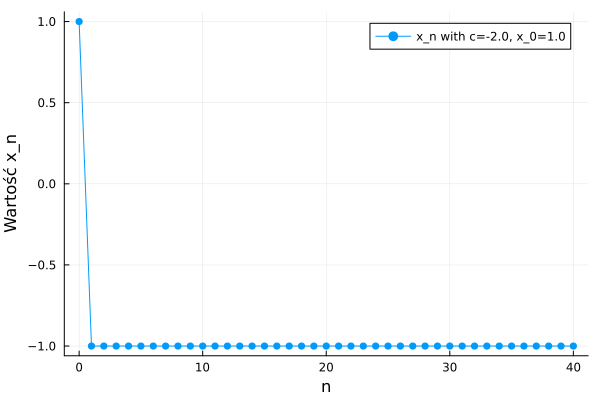
\includegraphics[width=\textwidth]{plot_1_1.png}
\caption{Wykres $x_{n + 1} = x_n^2 - 2$ z $x_0 = 1$.}
\end{figure}

\begin{figure}[H]
\centering
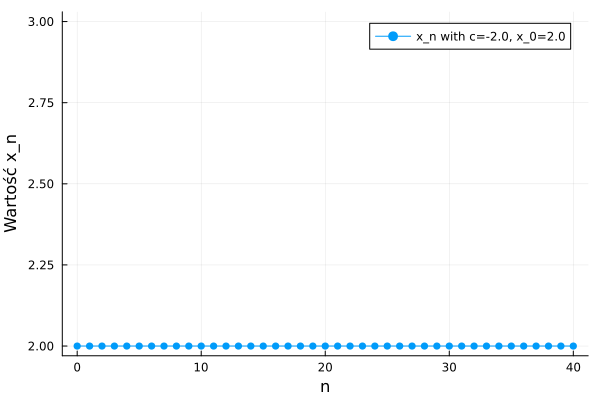
\includegraphics[width=\textwidth]{plot_1_2.png}
\caption{Wykres $x_{n + 1} = x_n^2 - 2$ z $x_0 = 2$.}
\end{figure}


\begin{figure}[H]
\centering
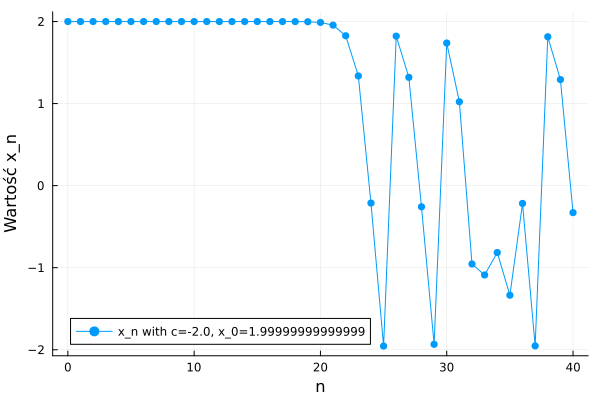
\includegraphics[width=\textwidth]{plot_1_3.png}
\caption{Wykres $x_{n + 1} = x_n^2 - 2$ z $x_0 = 1.99999999999999$.}
\end{figure}


\begin{figure}[H]
\centering
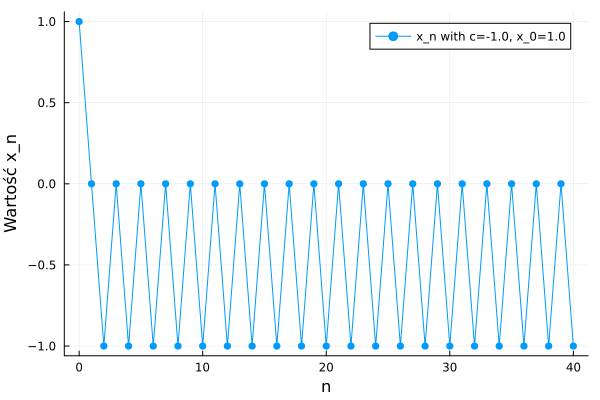
\includegraphics[width=\textwidth]{plot_2_1.png}
\caption{Wykres $x_{n + 1} = x_n^2 - 1$ z $x_0 = 1$.}
\end{figure}


\begin{figure}[H]
\centering
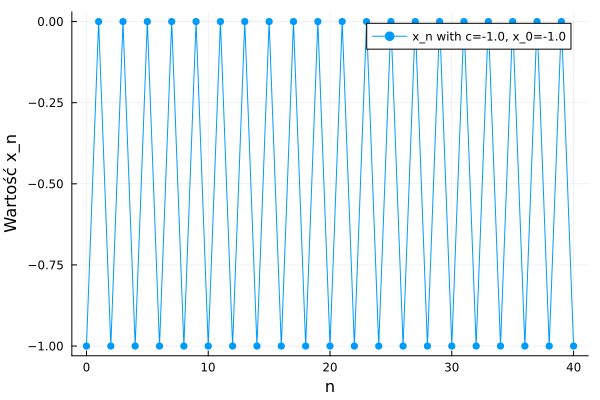
\includegraphics[width=\textwidth]{plot_2_2.png}
\caption{Wykres $x_{n + 1} = x_n^2 - 1$ z $x_0 = -1$.}
\end{figure}


\begin{figure}[H]
\centering
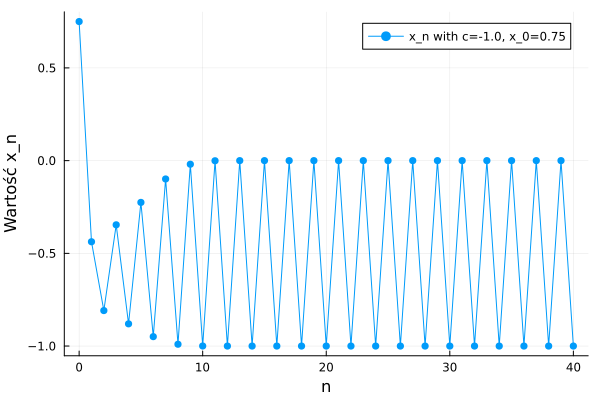
\includegraphics[width=\textwidth]{plot_2_3.png}
\caption{Wykres $x_{n + 1} = x_n^2 - 1$ z $x_0 = 0.75$.}
\end{figure}


\begin{figure}[H]
\centering
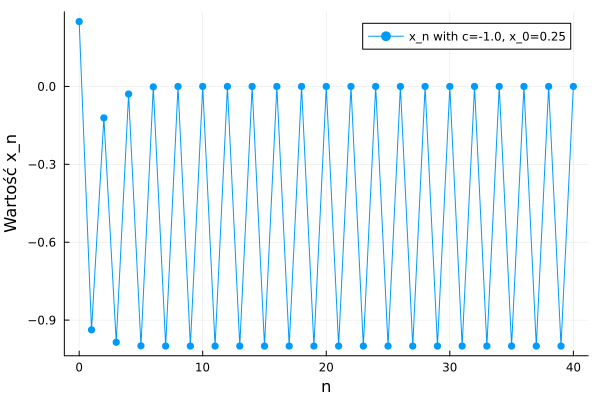
\includegraphics[width=\textwidth]{plot_2_4.png}
\caption{Wykres $x_{n + 1} = x_n^2 - 1$ z $x_0 = 0.25$.}
\end{figure}

\subsection{Obserwacje i wnioski}
Proces wyznaczania wartości $x_{n + 1} = x_n^2 - 2$ jest stabilny dla $x_0 \in \{1, 2\}$. Jednakże, dla minimalnie
mniejszego od 2 $x_0 = 1.99999999999999$ ciąg staje się chaotyczny, co wskazuje na niestabilność.

W przypadku $x_{n + 1} = x_n^2 - 1$ układy są stabilne dla każdego sprawdzonego $x_0$, ale stabilizacja następuje po
różnej ilości iteracji. Dla $x_0 \in \{1, -1\}$ dzieje się to od razu. Dla $x_0 = 0.75$ stabilizacja następuje dopiero
po 16 iteracjach, a dla $x_0 = 0.25$ po 11 iteracjach.

Widzimy, że dobór odpowiednich parametrów jest kluczowy w celu uzyskania zadowalająych wyników. Wpływają one na
stabilność układu, a także na tempo jego w stabilizacji w przypadku układów stabilnych.

\end{document}
